% Permission is granted to copy, distribute and/or modify this
% document under the terms of the Creative Common by-nc-sa License
% version 3.0 (CC BY-NC-SA 3.0). A copy of the license can be found at
% http://creativecommons.org/licenses/by-nc-sa/3.0/legalcode.

\documentclass[10pt,a4paper]{beamer}
\usepackage[french]{babel}
\usepackage{lmodern}
\usepackage[T1]{fontenc}
\usepackage[utf8]{inputenc}
\usepackage{UBdx}
\usepackage{graphicx}
\usepackage{datetime}
\usepackage{listings}
\usepackage[scaled]{helvet}
\usepackage[sorting=ydnt,backend=bibtex]{biblatex}
\addbibresource{biblio.bib}

\newdate{date}{30}{01}{2017}

\title{``A Wait-free Queue as Fast as Fetch-and-Add'' }
\subtitle{Chaoran~Yang, John Mellor-Crummey}

\author[L. Lucido]{Loris~Lucido\\[-.25em]}

\institute[IR]{Lecture d'articles - Soutenance}

\date{\displaydate{date}}

\begin{document}

\begin{frame}
  \vspace{3.5em}
  \titlepage
\end{frame}

%%%%%%%%%%%%%%%%%%%%%%%%%%%%%%%%%%%%%%%%%%%

\begin{frame}
  \frametitle{Progress guarantee of non-blocking object.}
  Blocking queue $\rightarrow$ unexpected delays from the Operating System
  can block every threads. \center \vfill
  \newtheorem{progress}[theorem]{Progress Guarantee}
  \begin{progress}
    \center
    \begin{columns}
      \begin{column}{0.3\textwidth}
      \end{column}
      \begin{column}{0.7\textwidth}
        \begin{itemize}
        \item[] An operation is guaranteed to end in a finite number of steps for\ldots
        \end{itemize}
      \end{column}
    \end{columns}
    \medskip
    \begin{columns}
      \begin{column}{0.3\textwidth}
        \begin{itemize}
        \item Obstruction-free
        \item Lock-free
        \item Wait-free
        \end{itemize}
      \end{column}
      \begin{column}{0.7\textwidth}
        \begin{itemize}
        \item[] 1 thread only (in isolation)
        \item[] at least 2 threads
        \item[] any number of threads
        \end{itemize}
      \end{column}
    \end{columns}
  \end{progress}
\end{frame}

\begin{frame}
  \frametitle{Implementation - Atomic primitives}
  \newtheorem{faa}[theorem]{Fetch-and-Add}
  \newtheorem{cas}[theorem]{Compare-and-Swap}
  \begin{faa}
    $FAA(x, v)$ returns the value of $x$ and increments it by $v$
  \end{faa}
  \vfill
  \begin{cas}
    $CAS(x,t,v)$ replaces $x$ by $v$ if $x$ equals $t$
  \end{cas}
\end{frame}

\begin{frame}
  \frametitle{Related works - queues}
  \small
  \begin{tabular}{|l|l|l|l|l|l|}\hline
    Queue & Progress & Primitive & Technique & Performance & Author \\\hline
    MS-Queue & Lock-free & CAS & \multicolumn{1}{|c|}{-} & CAS retry & M. M. Michael, \\
    & & & & & L. Scott \\\hline
    LCRQ & Lock-free & FAA and & FAA index & Fast & A. Morrison, \\
    & & CAS & & & Y. Afek \\\hline
    MS-queue & Wait-free & CAS & Fast-path- & CAS retry & A. Kogan,\\
    Wait-free ver. & & & slow-path & & E. Petrank \\\hline
    CC-queue & Blocking & SWAP & Combining & Blocking & P. Fatourou, \\
    & & & & & N. D. Kallimanis \\\hline
  \end{tabular}
\end{frame}

\begin{frame}
  \frametitle{Problematic}
  \large Can an \textbf{obstruction-free/lock-free} queue using
  \textbf{fetch-and-add} can be transformed to a \textbf{wait-free} queue using
  the \textbf{fast-path-slow-path} methodology ?
\end{frame}

\theoremstyle{example}
\newtheorem{algo}[theorem]{An obstruction-free queue using an infinite array.}
\begin{frame}[fragile]
  \frametitle{Obstruction-free queue}
  \begin{overprint}
  \onslide<1->\begin{algo}
    \begin{columns}
      \begin{column}{0.43\textwidth}
\begin{lstlisting}[mathescape, frame=single, label={lst:queue}, language=C, breaklines=true]
$\top$: invalid cell
$\bot$: empty cell
enqueue(x: var) {
  do t := FAA(&Tail, 1);
  while (!CAS(&Queue[t], $\bot$, x));
}
\end{lstlisting}
      \end{column}
      \begin{column}{0.55\textwidth}
\begin{lstlisting}[mathescape, frame=single, label={lst:queue}, language=C, breaklines=true]
dequeue(x: var) {
  do h := FAA(&Head, 1);
  while (CAS(&Queue[h], $\bot$, $\top$) and Tail > h);
  return (Queue[h] == $\top$ ? EMPTY : Queue[h]);
}
\end{lstlisting}
      \end{column}
    \end{columns}
  \end{algo}
\end{overprint}
\begin{overprint}
  \medskip
  \center
  \onslide<2> 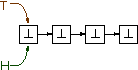
\includegraphics[scale=1.6]{img/q1.pdf}
  \onslide<3> 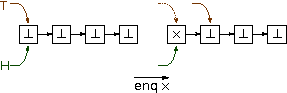
\includegraphics[scale=1.6]{img/q2.pdf}
  \onslide<4> 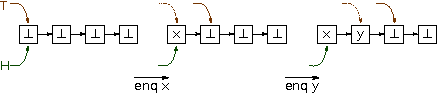
\includegraphics[scale=1.6]{img/q3.pdf}
  \onslide<5> 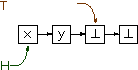
\includegraphics[scale=1.6]{img/q4.pdf}
  \onslide<6> 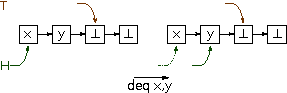
\includegraphics[scale=1.6]{img/q5.pdf}
  \onslide<7> 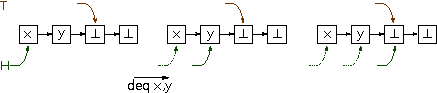
\includegraphics[scale=1.6]{img/q6.pdf}
  \onslide<8> 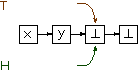
\includegraphics[scale=1.6]{img/q7.pdf}
  \onslide<9> 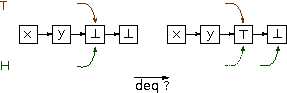
\includegraphics[scale=1.6]{img/q8.pdf}
\end{overprint}
\end{frame}

\begin{frame}
  \frametitle{Fast-path-slow-path methodology}
  \center
  Transform lock-free/obstruction-free queue into wait-free queue
  \vfill
  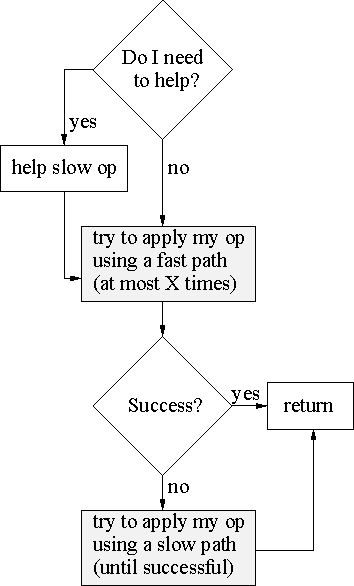
\includegraphics[scale=0.7]{../synthese/img/fpsp.pdf}
\end{frame}

\begin{frame}
  \frametitle{Results}
  \center
  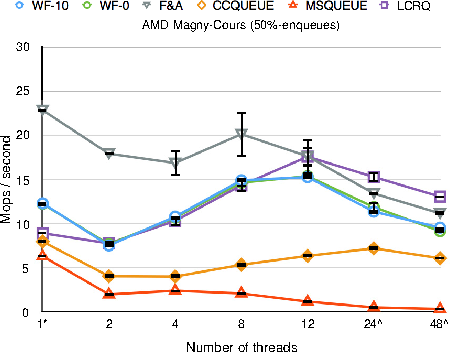
\includegraphics[scale=1.3]{../synthese/img/courbe.pdf}
\end{frame}

\begin{frame}
  \frametitle{Discussions}
  \begin{itemize}
  \item[] Some lock-free/blocking objects are \textit{practically} wait-free.
    \medskip
  \begin{itemize}
  \item 99.97\% enqueue done in one try on fast-path \medskip
  \item 95.95\% dequeue done in one try on fast-path
  \end{itemize}
  \vfill
\item[] Is fetch-and-add implemented in a starvation-free manner by the hardware
  ?
  \end{itemize}
\end{frame}

\begin{frame}
  \frametitle{Conclusion}
  \begin{itemize}
  \item First wait-free queue with performance as good as Lock-free queue \vfill
  \item Design complexity increased for wait-free queue \vfill
  \item Low probability of the worst-case scenario (slow-path)
\end{itemize}
\end{frame}

\begin{frame}[allowframebreaks]
 \frametitle{References}
 \nocite{*}
 \printbibliography
\end{frame}

\end{document}
